\begin{table}
	\centering
	\caption{Architectural component activity ratios formulas for Intel Ivy Bridge Architecture, inferred from Intel's 64 and IA-32 Architectures Software Developer's Manual \cite{fquesnel:progguide:intel10}}
	\label{tab:comp_formulas}
	\def\arraystretch{1.5}%
	\begin{tabular}{ | c | m{11cm} | } 
		\hline
		\textbf{Power Component} & \textbf{Componet Activity Formula} \\ 
		\hline
		\hline
		Fetch & UOPS\_RETIRED.ALL / CPU\_CLK\_UNHALTED.THREAD\_P \\ 
		\hline
		Branch Prediction Unit & BR\_INSTR\_RETIRED.ALL\_BRANCHES / CPU\_CLK\_UNHALTED.THREAD\_P \\ 
		\hline
		Arithmetic \& Logic Unit & (UOPS\_DISPATCHED\_PORT.PORT\_0 + UOPS\_DISPATCHED\_PORT.PORT\_1 + UOPS\_DISPATCHED\_PORT.PORT\_5) / CPU\_CLK\_UNHALTED.THREAD\_P \\ 
		\hline
		Floating Point & FP\_COMP\_OPS\_EXE.X87 / CPU\_CLK\_UNHALTED.THREAD\_P \\ 
		\hline
		L1 cache & L1D\_ALL.REF / CPU\_CLK\_UNHALTED.THREAD\_P \\ 
		\hline 
		L2 cache & (L2\_RQSTS.ALL\_RFO + L2\_RQSTS.ALL\_DEMAND\_DATA\_RD) / CPU\_CLK\_UNHALTED.THREAD\_P \\ 
		\hline	
		L3 cache & LLC.References / CPU\_CLK\_UNHALTED.THREAD\_P \\ 
		\hline
		Memory & LLC.Misses / CPU\_CLK\_UNHALTED.THREAD\_P \\ 
		\hline
	\end{tabular}
	\vspace{.5cm}
\end{table}

\begin{figure}[ht!]
	\centering
  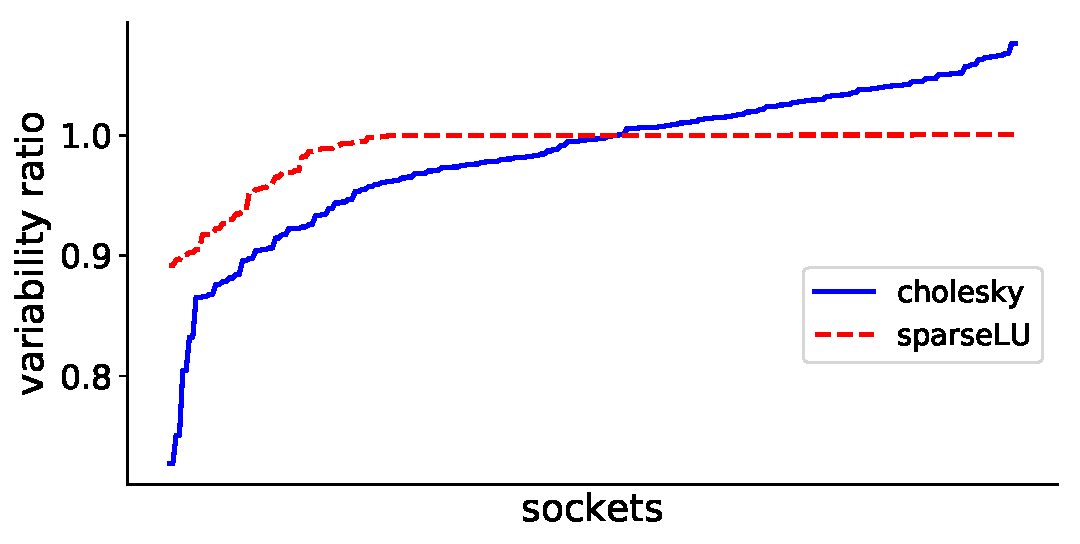
\includegraphics[width=.8\textwidth]{power_aware_job_scheduling/figures/benchmark_var_comparison}
	\caption{Comparison between the variability ratios over all 256 sockets as observed for \textit{cholesky} and \textit{sparseLU} benchmarks.  The cpu bound \textit{cholesky} detects variability more precisely than \textit{sparseLU}.}
	\label{fig:bench_var_comparison}
	\vspace{.5cm}
\end{figure}


%Power consumption variability across same die technology chips is a result of differing leakage power caused by material differences within the individual wafers~\cite{Teodorescu:2008:VAS:1381306.1382152,4798265,Borkar:2003:PVI:775832.775920,Rountree:2012:BDF:2357488.2357648}.  This variation affects transistor threshold voltage ($V_{th}$) and effective
%channel length ($V_{Eff}$)~\cite{Totoni:tech:2014}, which in turn determines transistor leakage.  At architectural level, any architectural component of a chip can be influenced.
Power modeling has received a lot of attention from researchers and developers as it provides a quick and robust way to understand the power behavior of a system.  
A common approach for predicting power consumption consists in the usage of 
Performance Monitoring Counters (PMC)~\cite{Bertran:2010:DRP:1810085.1810108,Singh:2009:RTP:1577129.1577137,Bellosa:2000:BED:566726.566736,4211032,Bircher:2005:RIM:1077603.1077668,Li:2003:RME:781027.781048},
since sampling PMC does not introduce significant power interference~\cite{Joseph:2001:RPE:383082.383119,Isci:2003:RPM:956417.956567}
and PMC-based prediction models decompose a chip into several components in terms of power consumption~\cite{Bertran:2010:DRP:1810085.1810108}.
While power prediction models are employed to find the best tradeoff between power and performance~\cite{Gholkar:2016:PTH:2967938.2967961},
we are not aware of any previous work that uses variability-aware power models to guide job scheduling decisions.  

In the rest of the document, we consider a cluster to consist of multiple nodes, each with multiple sockets. Thus, the terms socket and CPU are used interchangeably.

\subsection{Power Ratio Model}
\label{sec:naive_model}

Our first (baseline) model attempts to circumvent the relative complexity of dealing with a PMC-based model by assuming that all applications are impacted by manufacturing variability in the same way.  
It considers a single benchmark application, in our case an OpenMP implementation of the \textit{cholesky} decomposition of a dense 65 MB matrix, 
and measures its average power consumption on each socket we want to generate a model for.
We chose cholesky because it is a dense linear algebra kernel, which stresses both CPU and cache memory accounting for power consumption variability across the sockets.
%#in our case an OpenMP implementation of the \textit{cholesky} decomposition of a dense 65 MB matrix, 
Once this information is obtained, we characterize the variability between sockets in terms of power ratios and we apply them to power measurements of a target application (denoted as $app$) obtained from an execution on a single reference socket (denoted as $socket_{ref}$).
% of the application we want to make predictions for . 
The power consumption of $app$ on any $socket_i$ is then computed by the following formula:

\begin{equation}
\label{eq:naive_model}
P_{socket_{i}}^{app} = P_{socket_{ref}}^{app} * \frac{P_{socket_{i}}^{choleksy}}{P_{socket_{ref}}^{cholesky}}
\end{equation}

In the case of multi-node applications, we predict the power consumption of each socket an MPI process run on, by applying the power ratio corresponding to that socket.

A limitation of the PR model is that it's precision is subject to the benchmark application used
for measuring the sockets' manufacturing variability.  Figure \ref{fig:bench_var_comparison} shows
the manufacturing variability for two distinct benchmarks, \textit{cholesky} and \textit{sparseLU},
as measured by running them on all sockets.  As observer, the two benchmarks produce different
variability ratios.  In the case of \textit{sparseLU}, which solves the LU factorization problem
on a sparse matric, the observed variability ratio is on many occasions 1.  This means that this
benchmark fails to measure manufacturing variability effectively and would be able to adjust
the original prediction to fit a socket's variability.  On the other hand, \textit{cholesky},
which is a computation bound application and stresses the processor more than \textit{sparseLU},
produces a more precise view of the system's heterogeneity due to manufacturing variability.


\subsection{PMC-based Prediction Models}
\label{sec:pmcs_model}
Our second model is based on PMC data and aims at capturing the impact of manufacturing variability on the execution of a particular application on power-capped sockets. 
Specifically, it uses PMC values to capture the contribution of each chip's architectural components to power consumption and then models each component using activity ratios.
These ratios are defined as the number of retired micro operations relevant for the targeted architectural component per active cycle.  
%For cores, the activity ratio is the number of active cores at a given moment.  
For example, for main memory and caches, activity ratios are the number of references or misses per cycle, respectively. 
Activity ratios reflect the usage of the corresponding component for a given application.  The model assumes that a component's contribution to power consumption is proportionate
to its usage (activity ratio).
The granularity at which we can decompose a chip into architectural components depends on the underlying architecture and the available PMC.    
Table~\ref{tab:comp_formulas} shows the different components and their corresponding PMC formulas for the Intel's Ivy Bridge architecture.  
We infer the 
formulas from the Intel 64 and IA-32 Architectures Software Developer's Manual~\cite{fquesnel:progguide:intel10}.

\begin{figure*}[p]
	\centering
	\begin{subfigure}[b]{.48\textwidth}
  	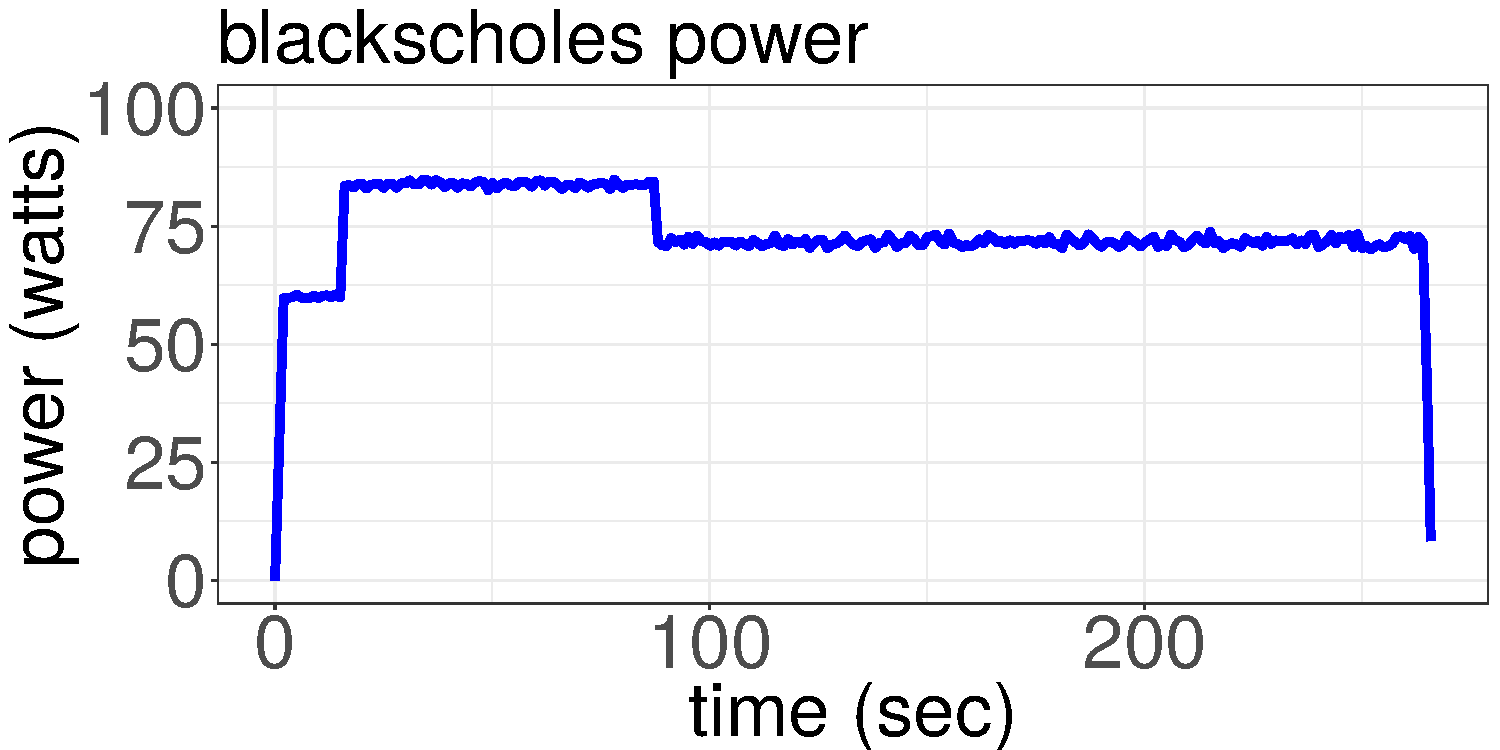
\includegraphics[width=\textwidth]{power_aware_job_scheduling/figures/activity_ratios/blackscholes_pkg_power}
  \end{subfigure}%
~
	\begin{subfigure}[b]{.48\textwidth}
  	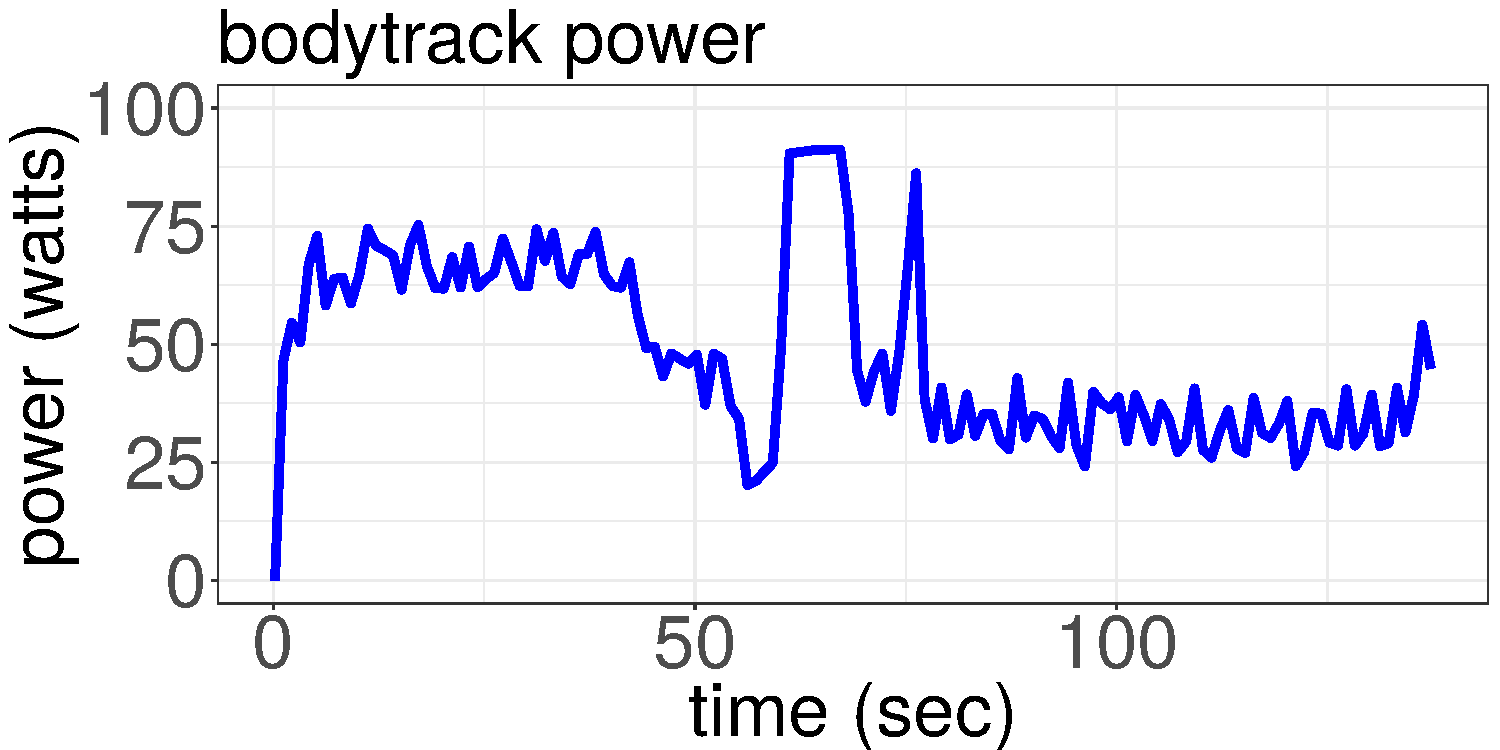
\includegraphics[width=\textwidth]{power_aware_job_scheduling/figures/activity_ratios/bodytrack_pkg_power}
	\end{subfigure}%
	\vspace{0.1cm}
	\begin{subfigure}[b]{.48\textwidth}
  	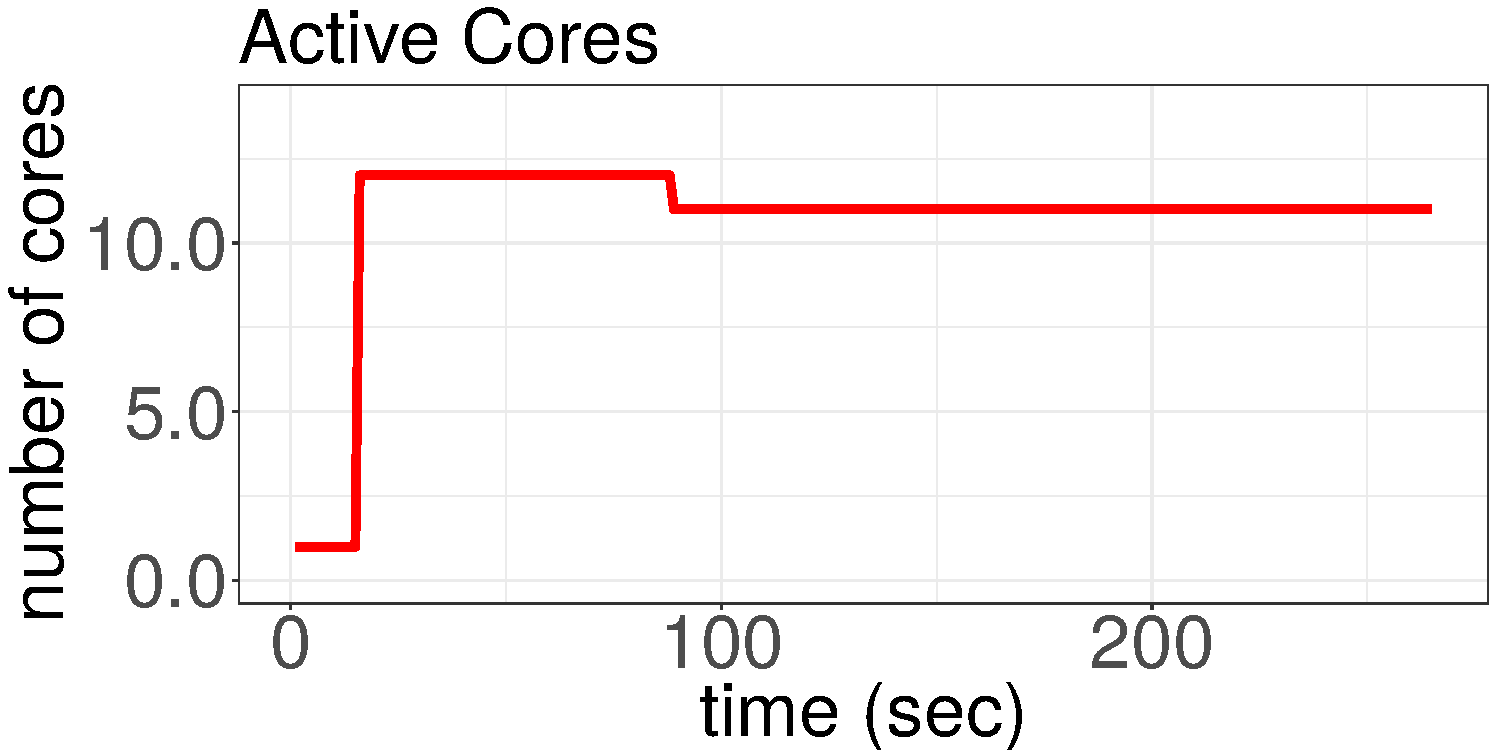
\includegraphics[width=\textwidth]{power_aware_job_scheduling/figures/activity_ratios/blackscholes_CORES}
  \end{subfigure}%
~
	\begin{subfigure}[b]{.48\textwidth}
  	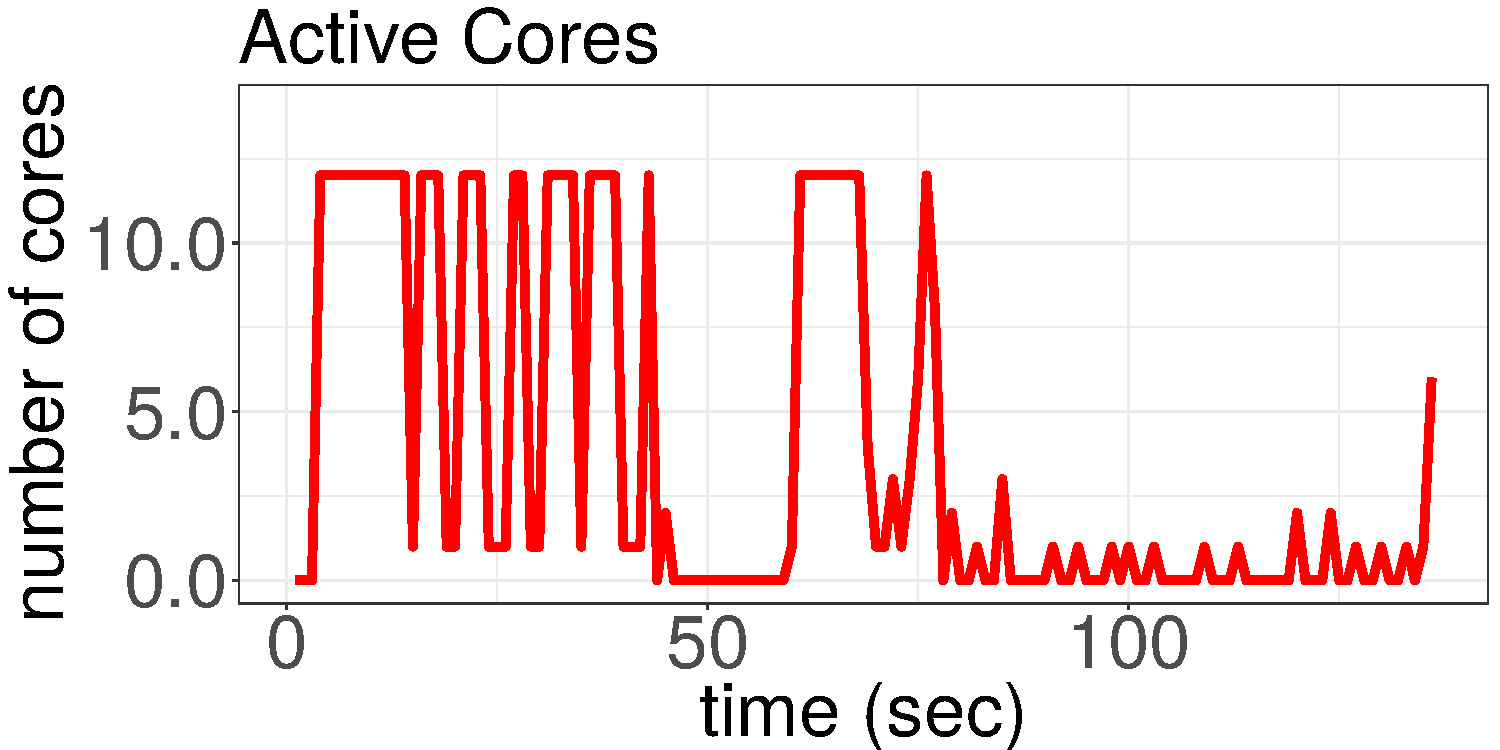
\includegraphics[width=\textwidth]{power_aware_job_scheduling/figures/activity_ratios/bodytrack_CORES}
  \end{subfigure}%
	\vspace{0.1cm}
	\begin{subfigure}[b]{.48\textwidth}
  	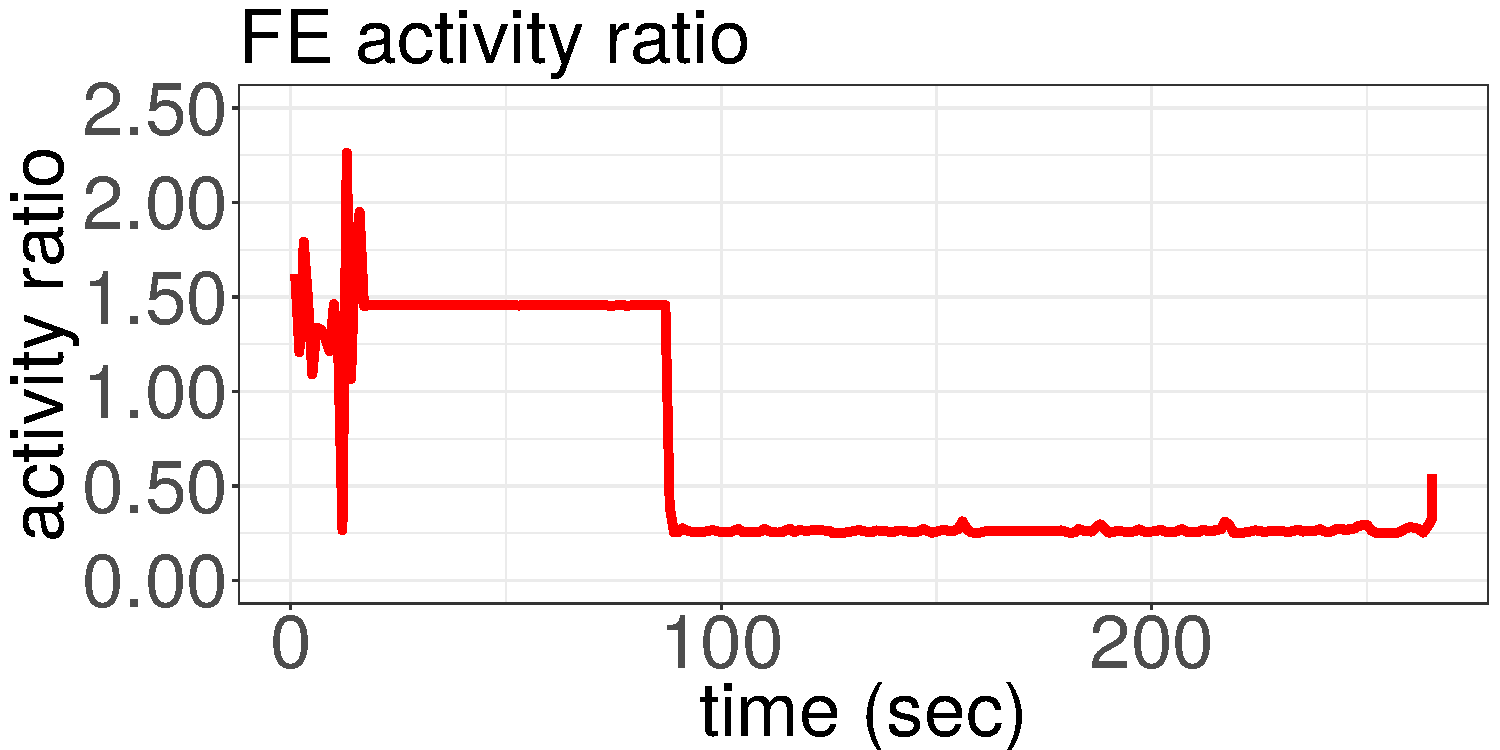
\includegraphics[width=\textwidth]{power_aware_job_scheduling/figures/activity_ratios/blackscholes_IPC}
  \end{subfigure}%
~
	\begin{subfigure}[b]{.48\textwidth}
  	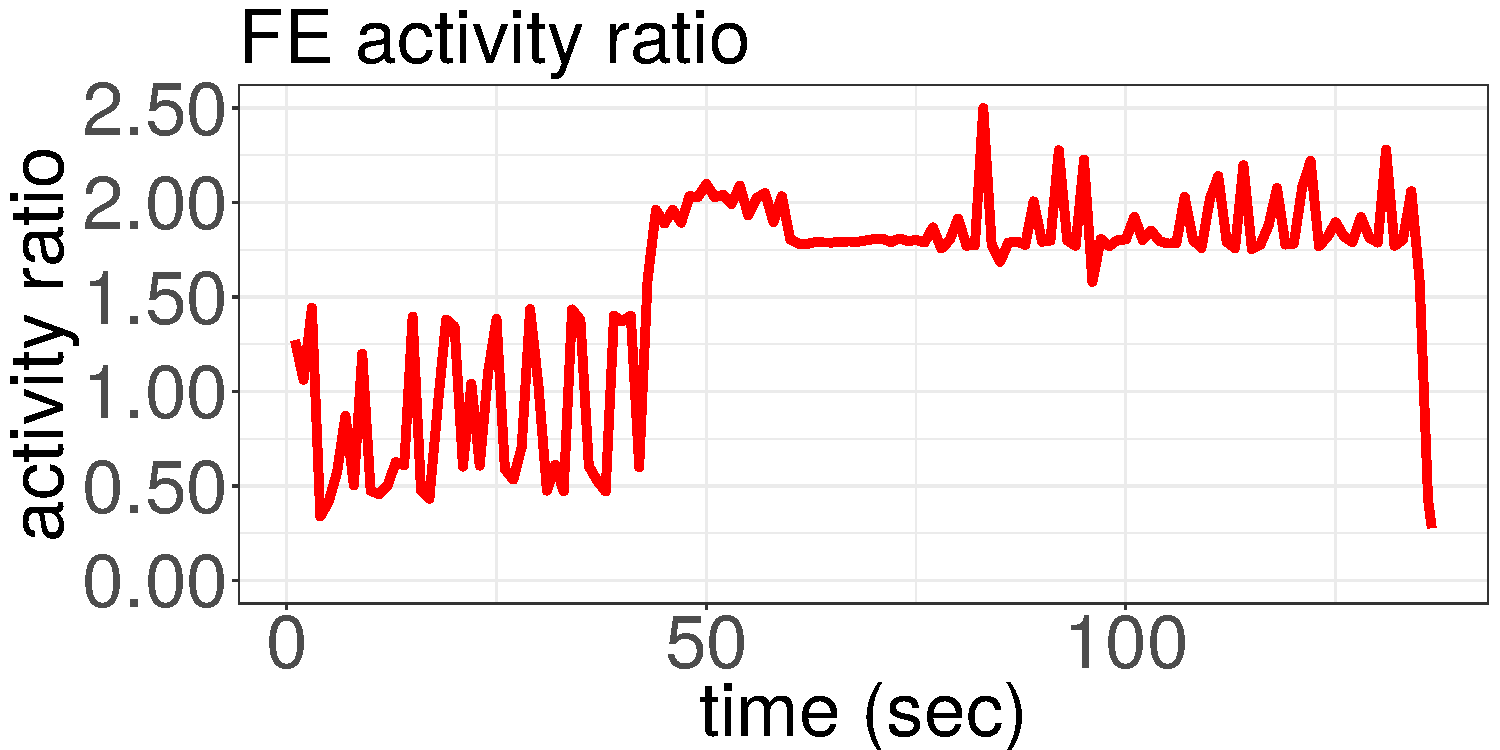
\includegraphics[width=\textwidth]{power_aware_job_scheduling/figures/activity_ratios/bodytrack_IPC}
  \end{subfigure}%
	\vspace{0.1cm}
	\begin{subfigure}[b]{.48\textwidth}
  	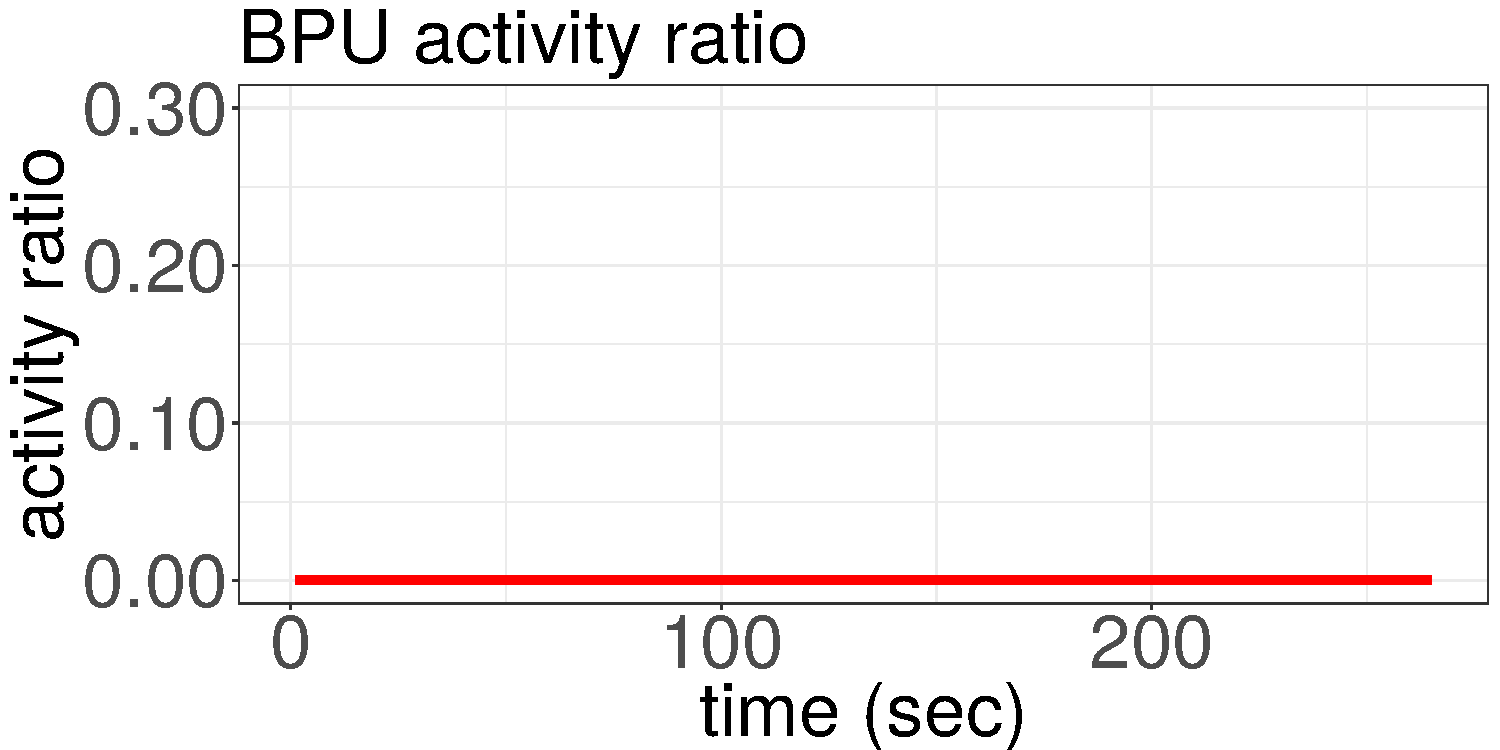
\includegraphics[width=\textwidth]{power_aware_job_scheduling/figures/activity_ratios/blackscholes_BPU}
  \end{subfigure}%
~
	\begin{subfigure}[b]{.48\textwidth}
  	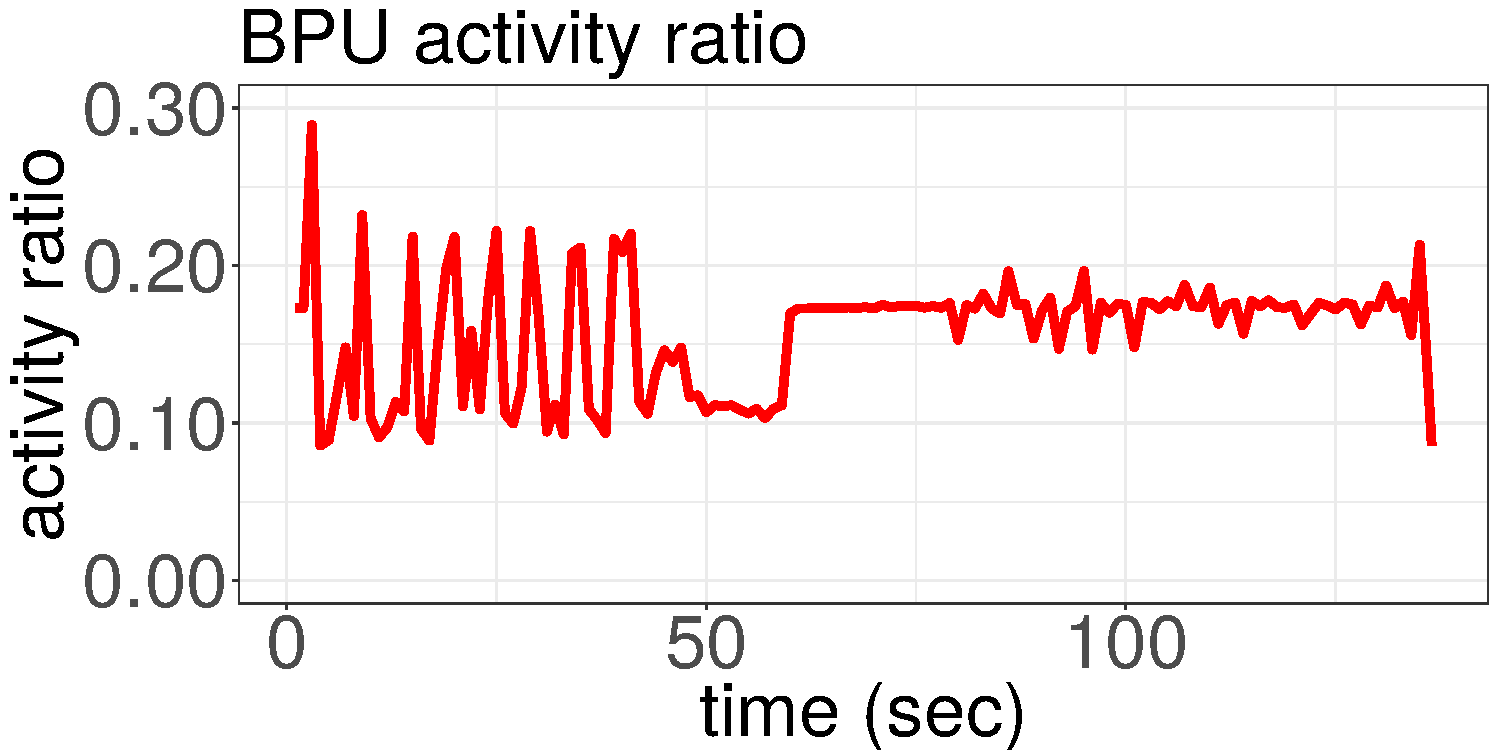
\includegraphics[width=\textwidth]{power_aware_job_scheduling/figures/activity_ratios/bodytrack_BPU}
  \end{subfigure}%
	\vspace{0.1cm}
	\begin{subfigure}[b]{.48\textwidth}
  	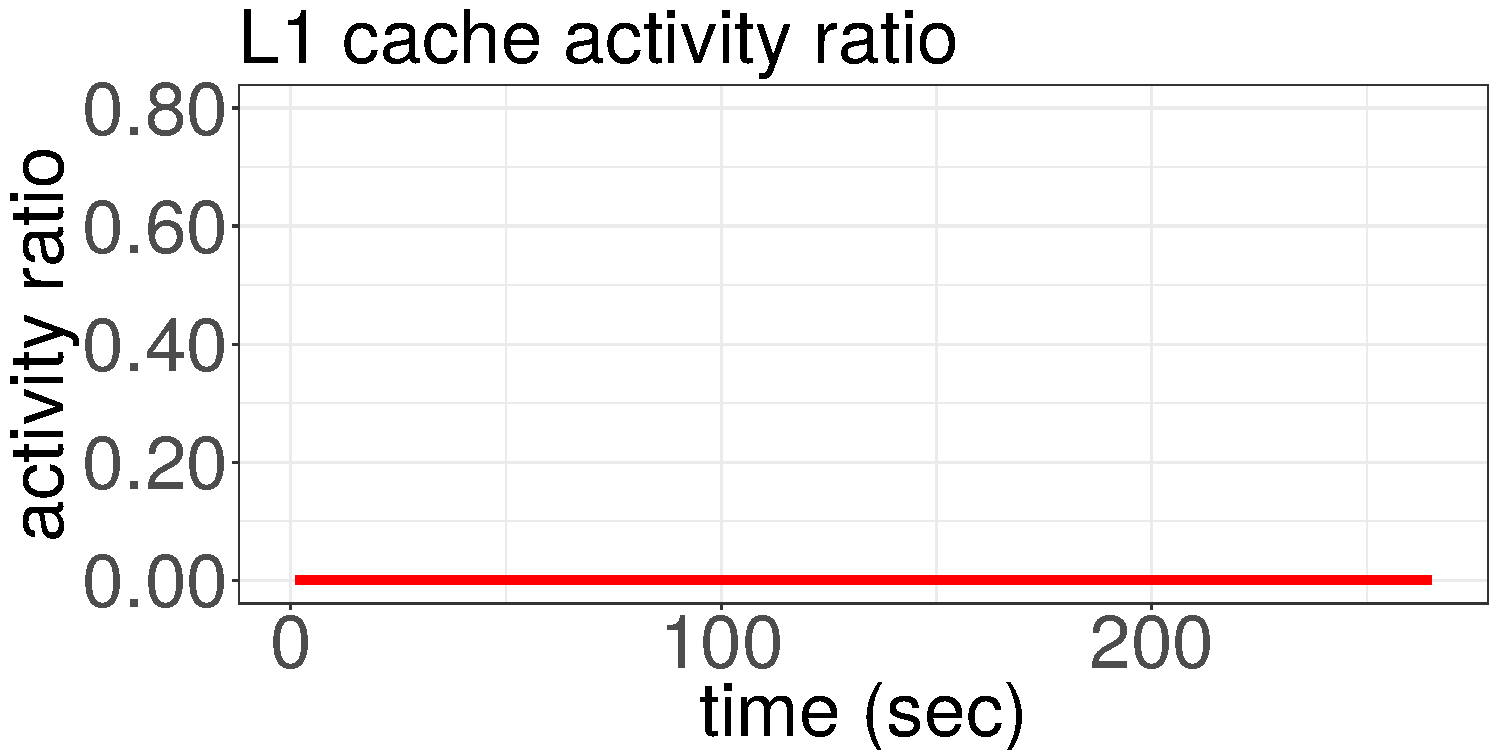
\includegraphics[width=\textwidth]{power_aware_job_scheduling/figures/activity_ratios/blackscholes_L1}
  \end{subfigure}%
~
	\begin{subfigure}[b]{.48\textwidth}
  	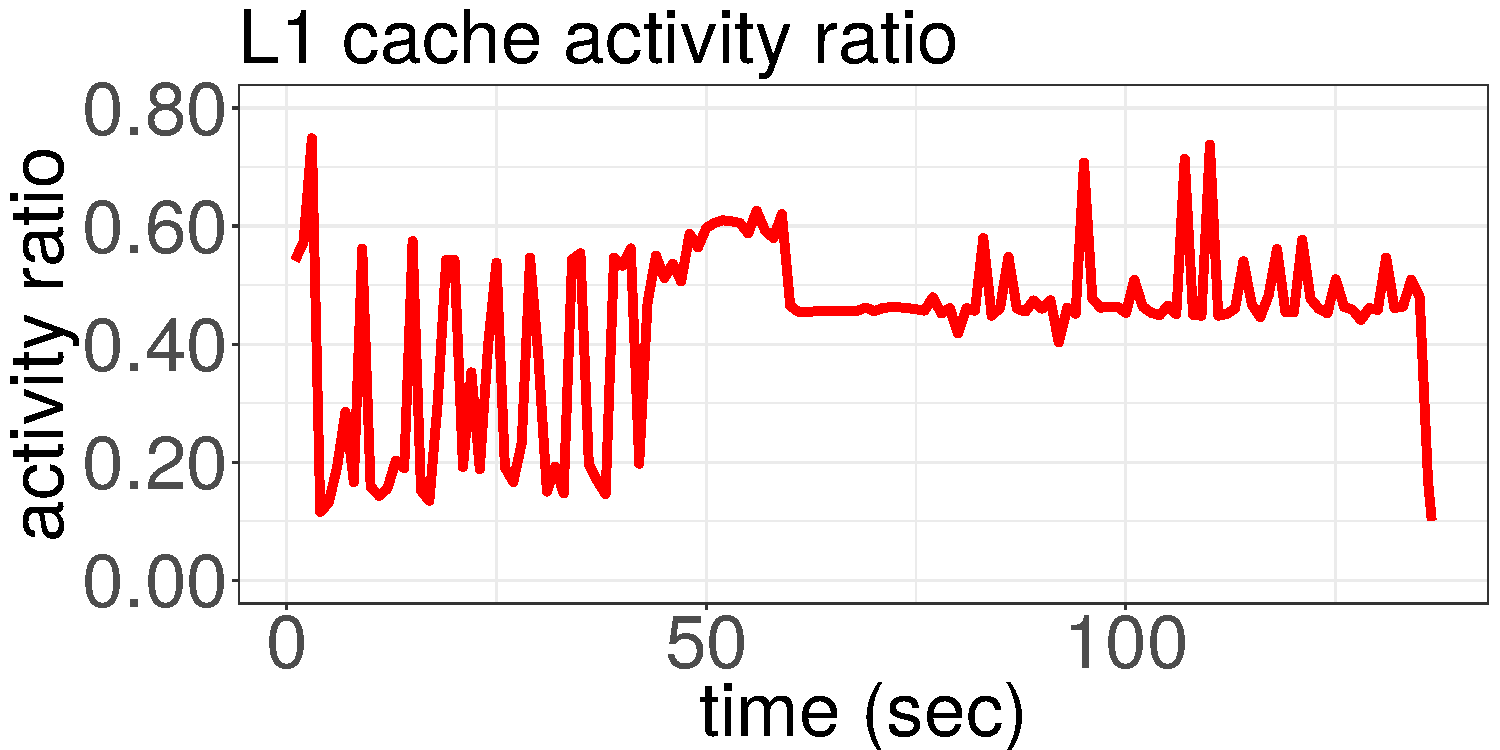
\includegraphics[width=\textwidth]{power_aware_job_scheduling/figures/activity_ratios/bodytrack_MEM}
  \end{subfigure}%
	\caption{Power, active cores and component activity ratio traces when running on 12 cores of a single socket.  Architectural components shown are the fetch unit (FE), branch prediction unit (BPU)
					and L1 cache.  The activity ratios are the number of retired micro operations per unhalted cycle, relevant to each architectural component.
					In the case of cores, activity ratio is the number of active cores.  For memory the activity ratio is measured as the number of references (for caches) or LLC misses (for main memory) per cycle.
					For multi-node applications, we show the activity on the socket running one the MPI processes.  PMC data is collected for all the processes and individual predictions are made for each socket.}
	\label{fig:component_activity_ratios_single_node}
	\vspace{.5cm}
\end{figure*}

\begin{figure*}[p]
	\centering
	\begin{subfigure}[b]{.48\textwidth}
	  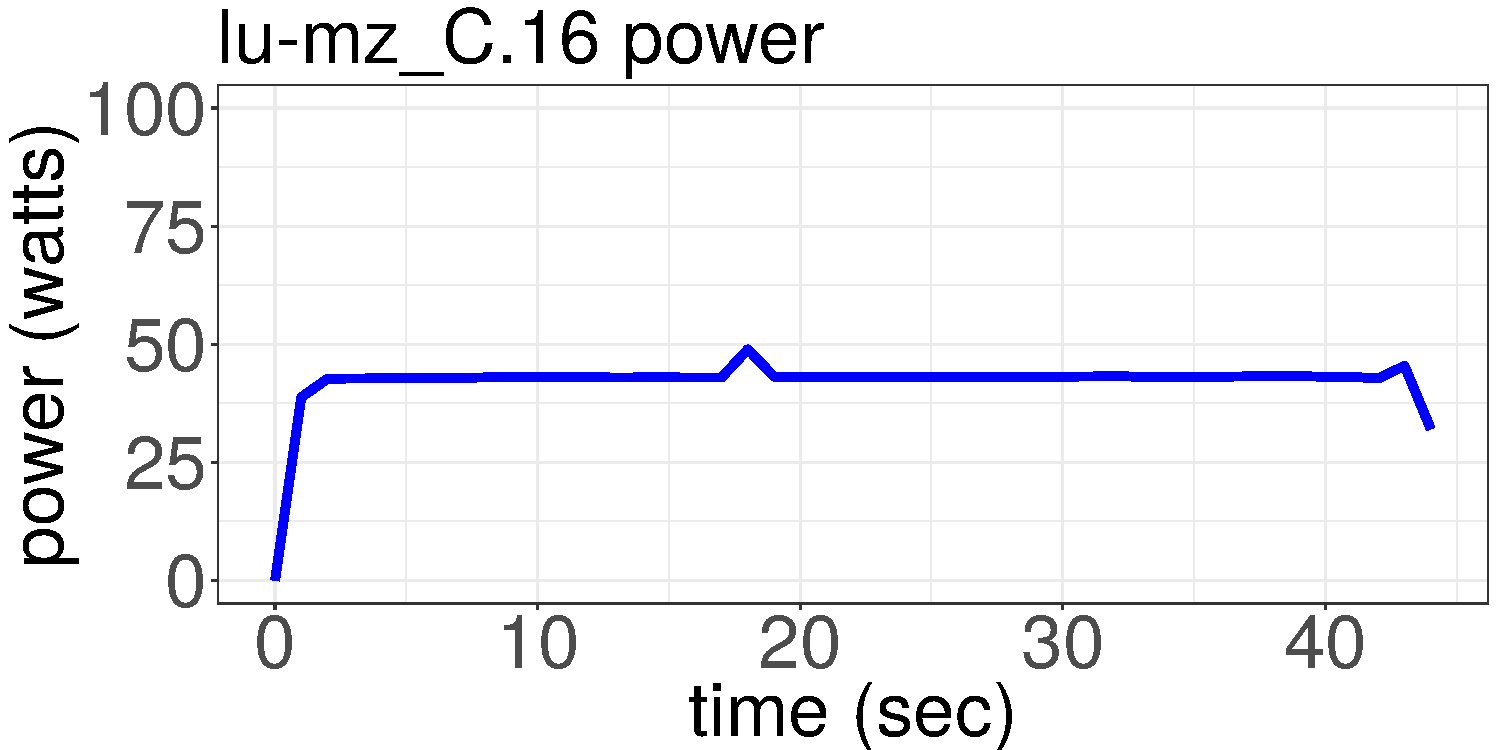
\includegraphics[width=\textwidth]{{power_aware_job_scheduling/figures/activity_ratios/lu-mz_C.16_pkg_power}.pdf}
	\end{subfigure}%
~
	\begin{subfigure}[b]{.48\textwidth}
	  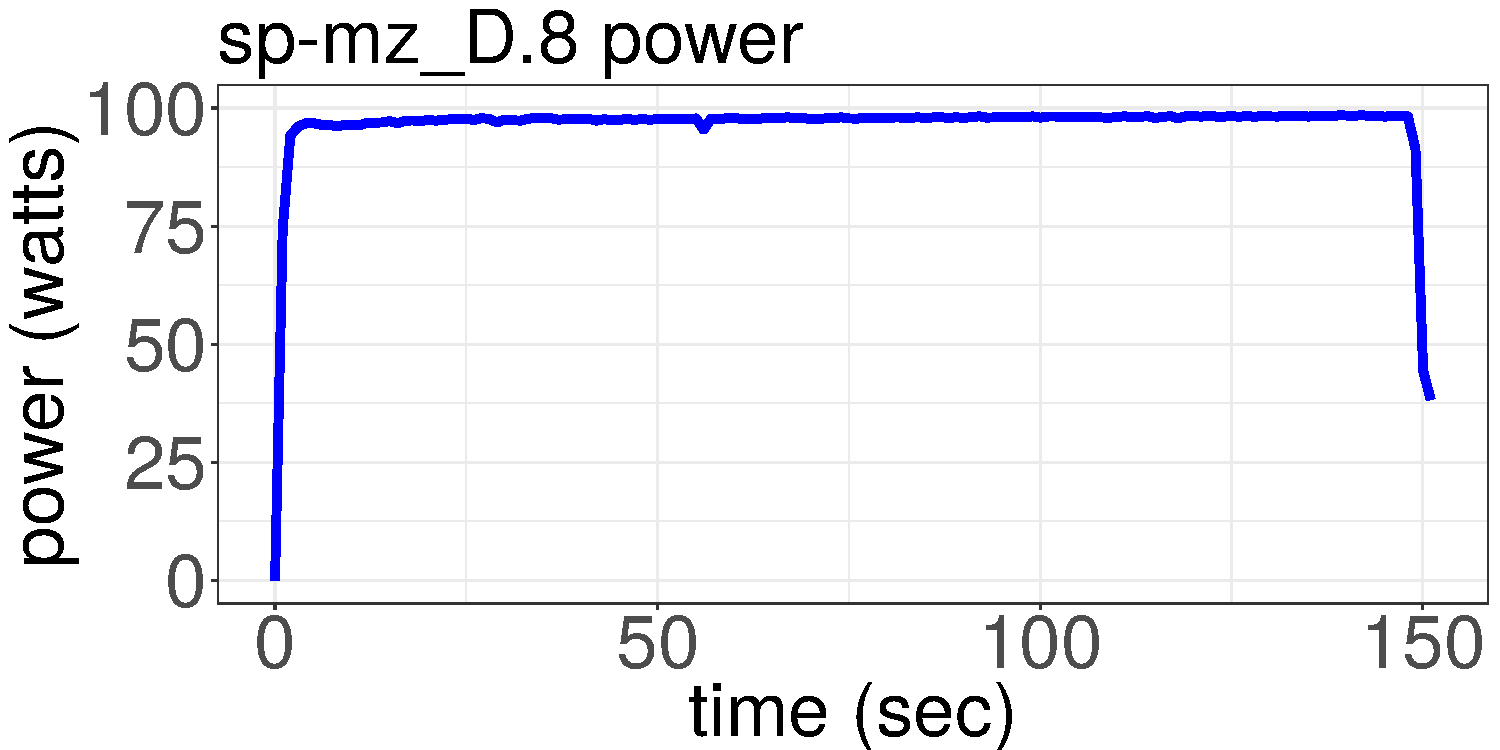
\includegraphics[width=\textwidth]{{power_aware_job_scheduling/figures/activity_ratios/sp-mz_D.8_pkg_power}.pdf}
	\end{subfigure}%
	\vspace{0.1cm}
	\begin{subfigure}[b]{.48\textwidth}
	  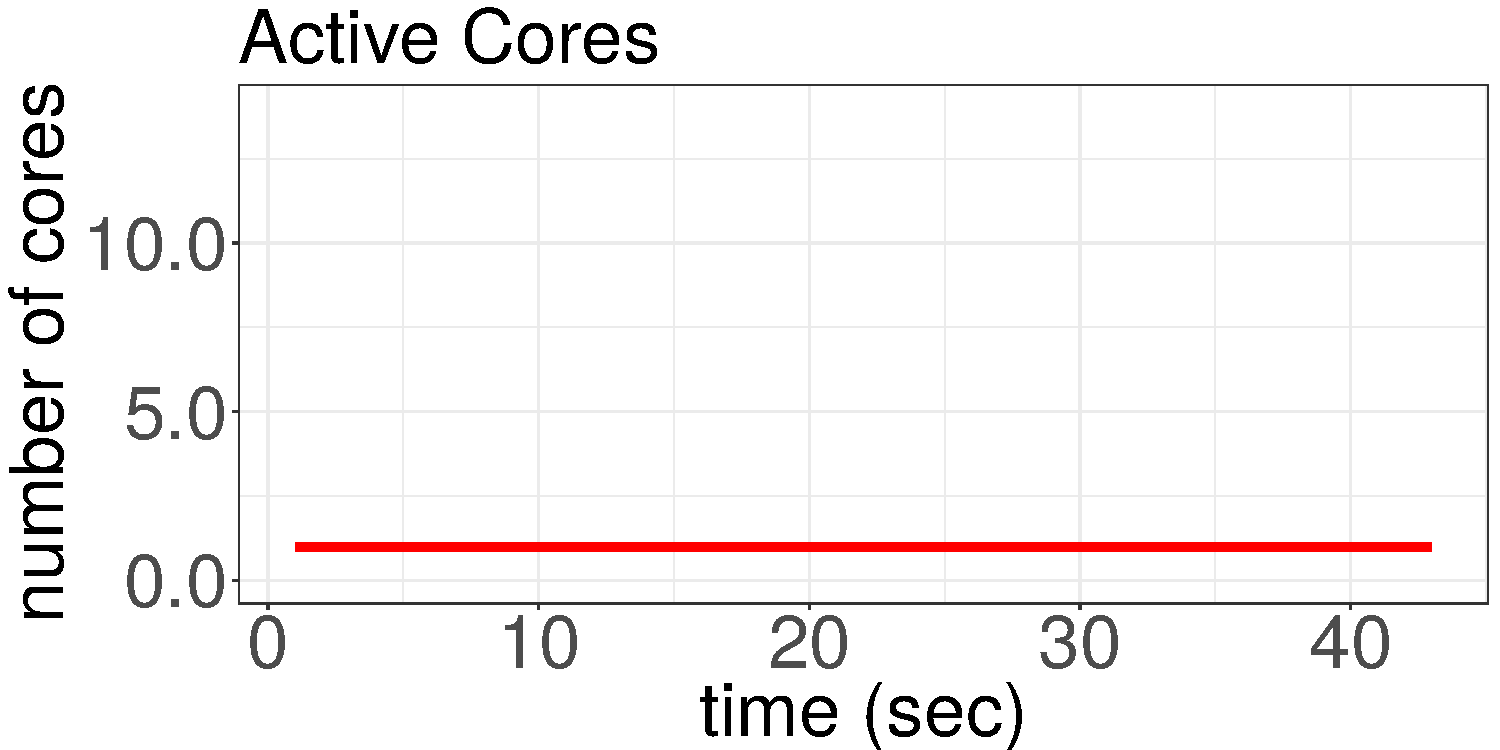
\includegraphics[width=\textwidth]{{power_aware_job_scheduling/figures/activity_ratios/lu-mz_C.16_CORES}.pdf}
	\end{subfigure}%
~
	\begin{subfigure}[b]{.48\textwidth}
	  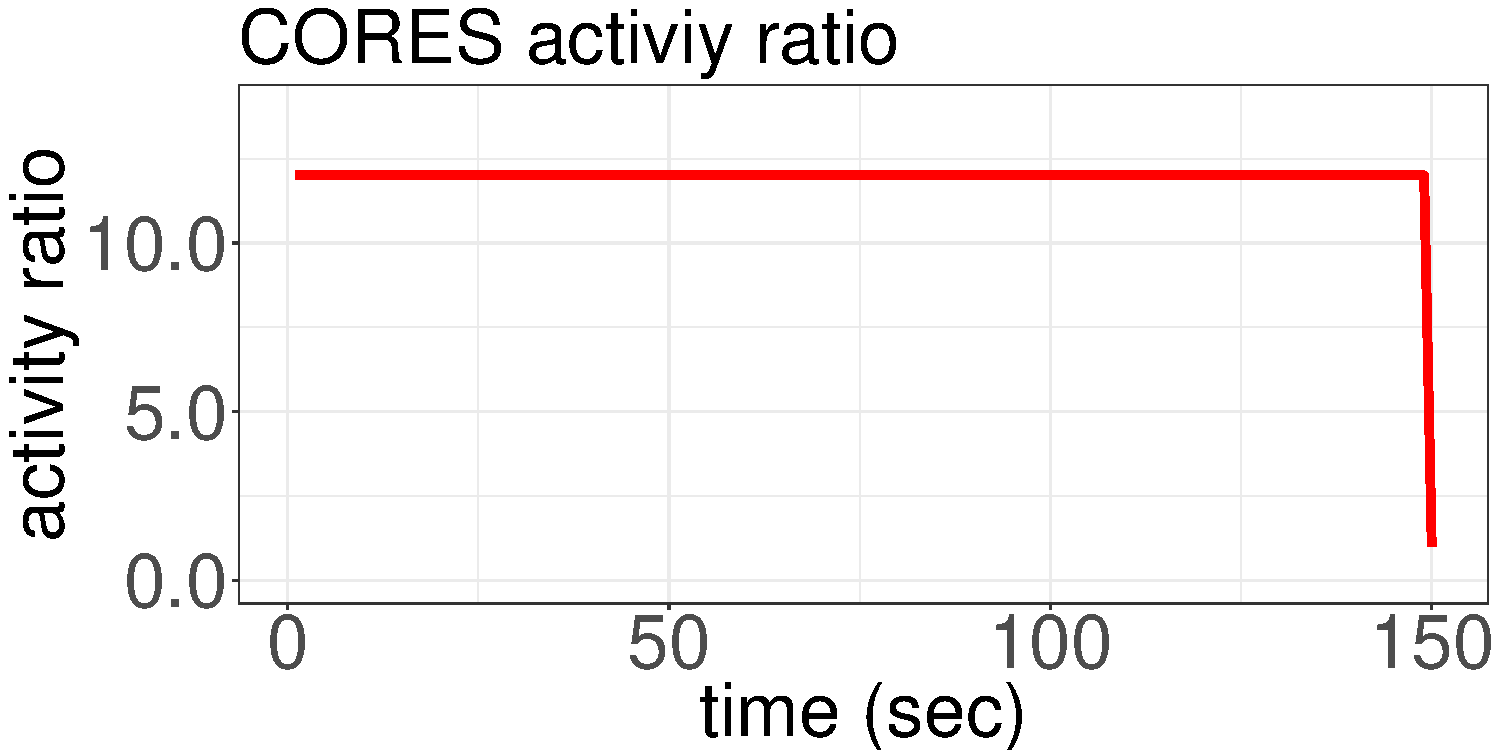
\includegraphics[width=\textwidth]{{power_aware_job_scheduling/figures/activity_ratios/sp-mz_D.8_CORES}.pdf}
	\end{subfigure}%
	\vspace{0.1cm}
	\begin{subfigure}[b]{.48\textwidth}
	  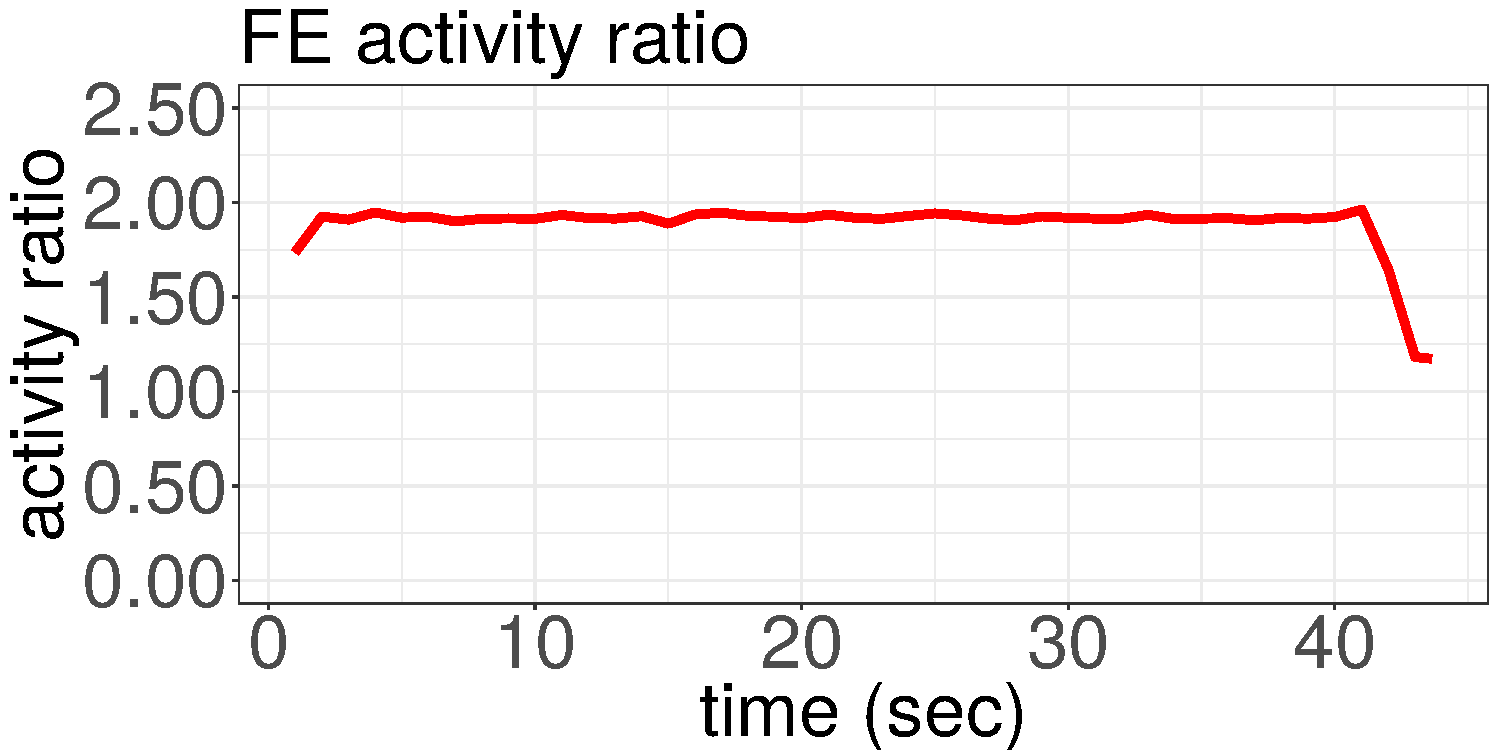
\includegraphics[width=\textwidth]{{power_aware_job_scheduling/figures/activity_ratios/lu-mz_C.16_IPC}.pdf}
	\end{subfigure}%
~
	\begin{subfigure}[b]{.48\textwidth}
	  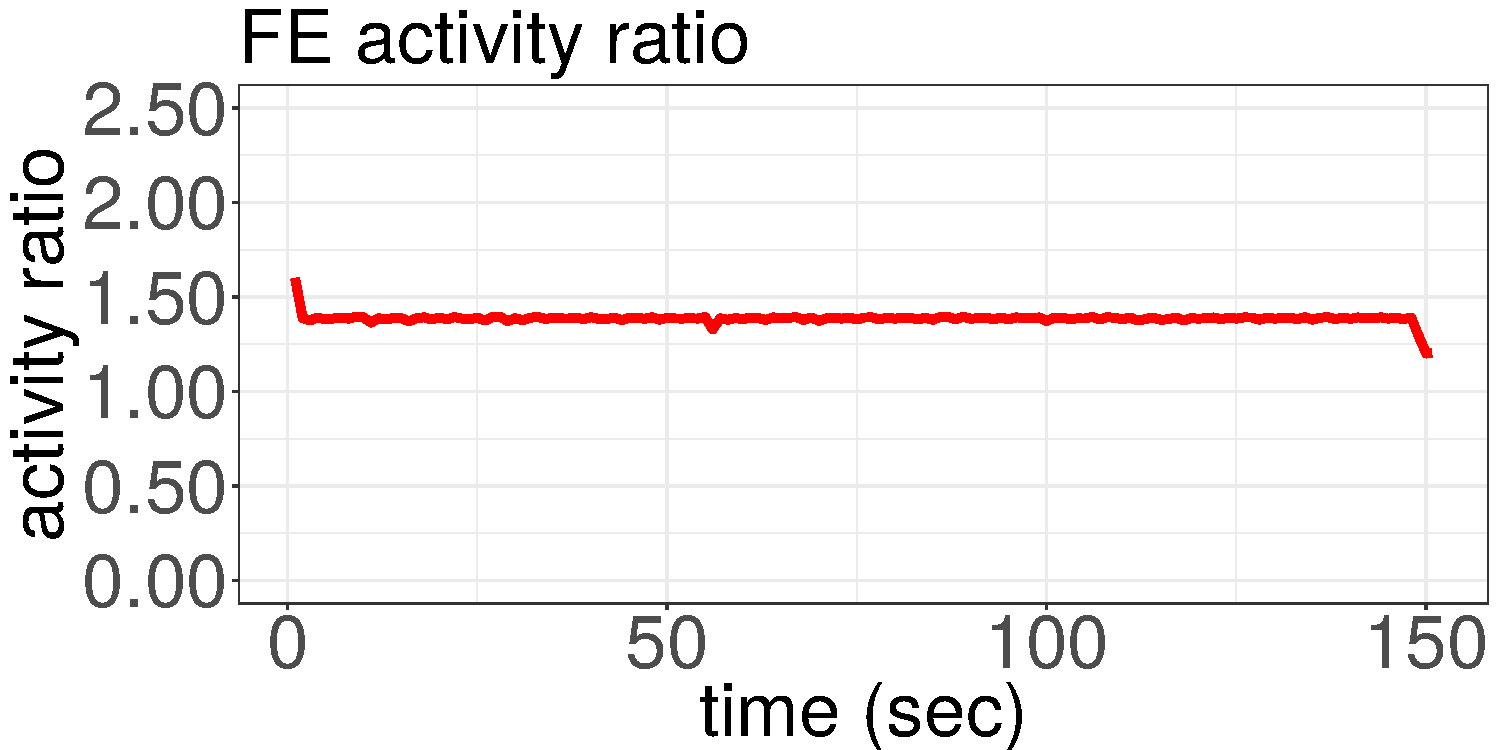
\includegraphics[width=\textwidth]{{power_aware_job_scheduling/figures/activity_ratios/sp-mz_D.8_IPC}.pdf}
	\end{subfigure}%
	\vspace{0.1cm}
	\begin{subfigure}[b]{.48\textwidth}
	  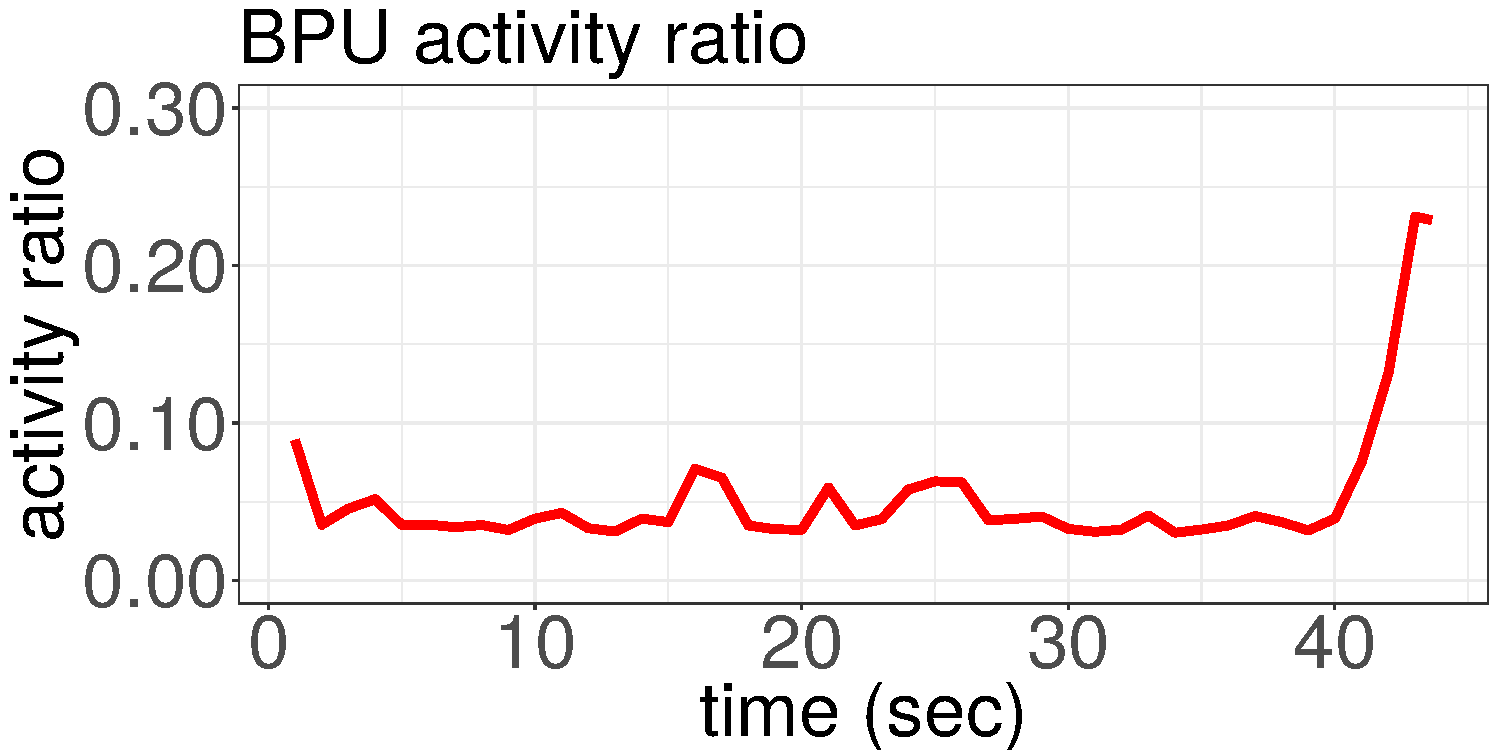
\includegraphics[width=\textwidth]{{power_aware_job_scheduling/figures/activity_ratios/lu-mz_C.16_BPU}.pdf}
	\end{subfigure}%
~
	\begin{subfigure}[b]{.48\textwidth}
	  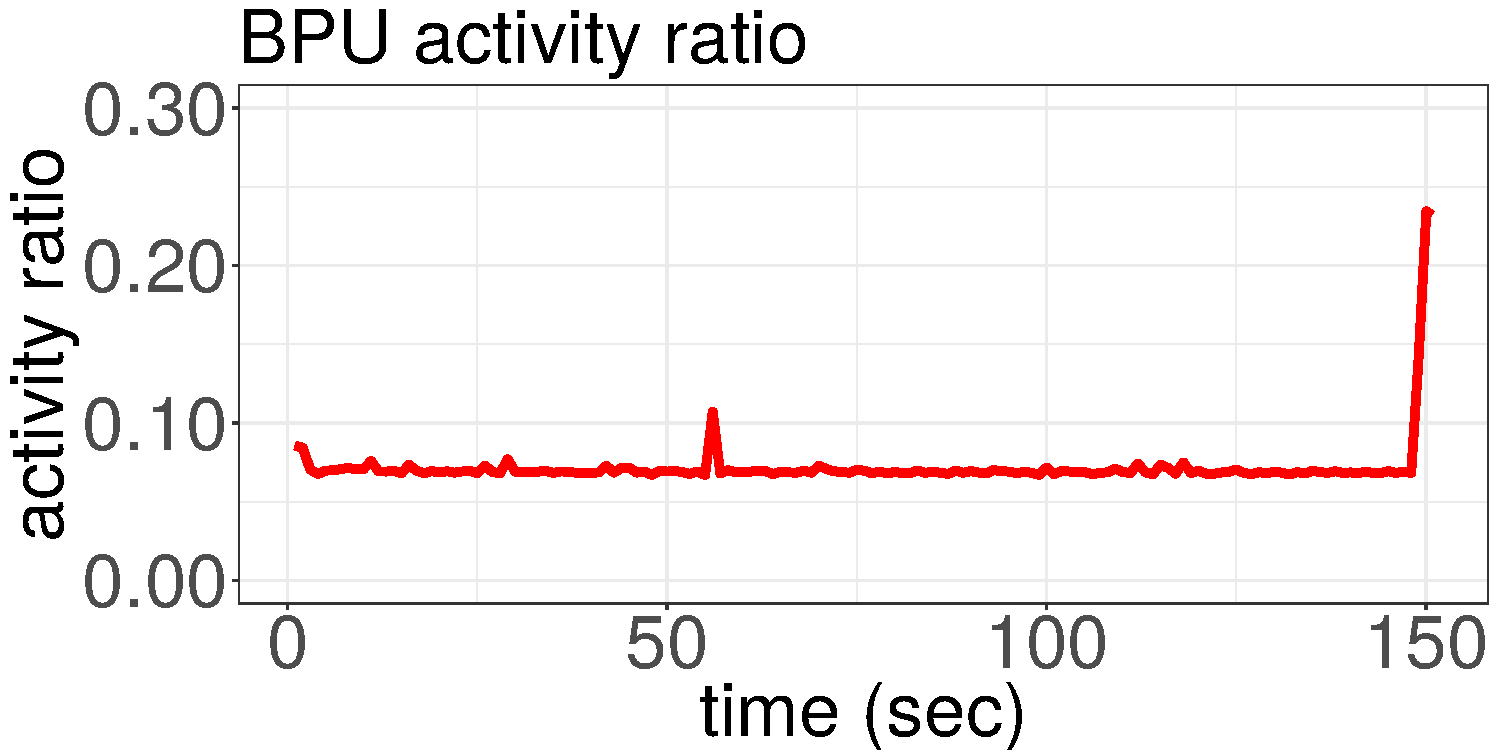
\includegraphics[width=\textwidth]{{power_aware_job_scheduling/figures/activity_ratios/sp-mz_D.8_BPU}.pdf}
	\end{subfigure}%
	\vspace{0.1cm}
	\begin{subfigure}[b]{.48\textwidth}
	  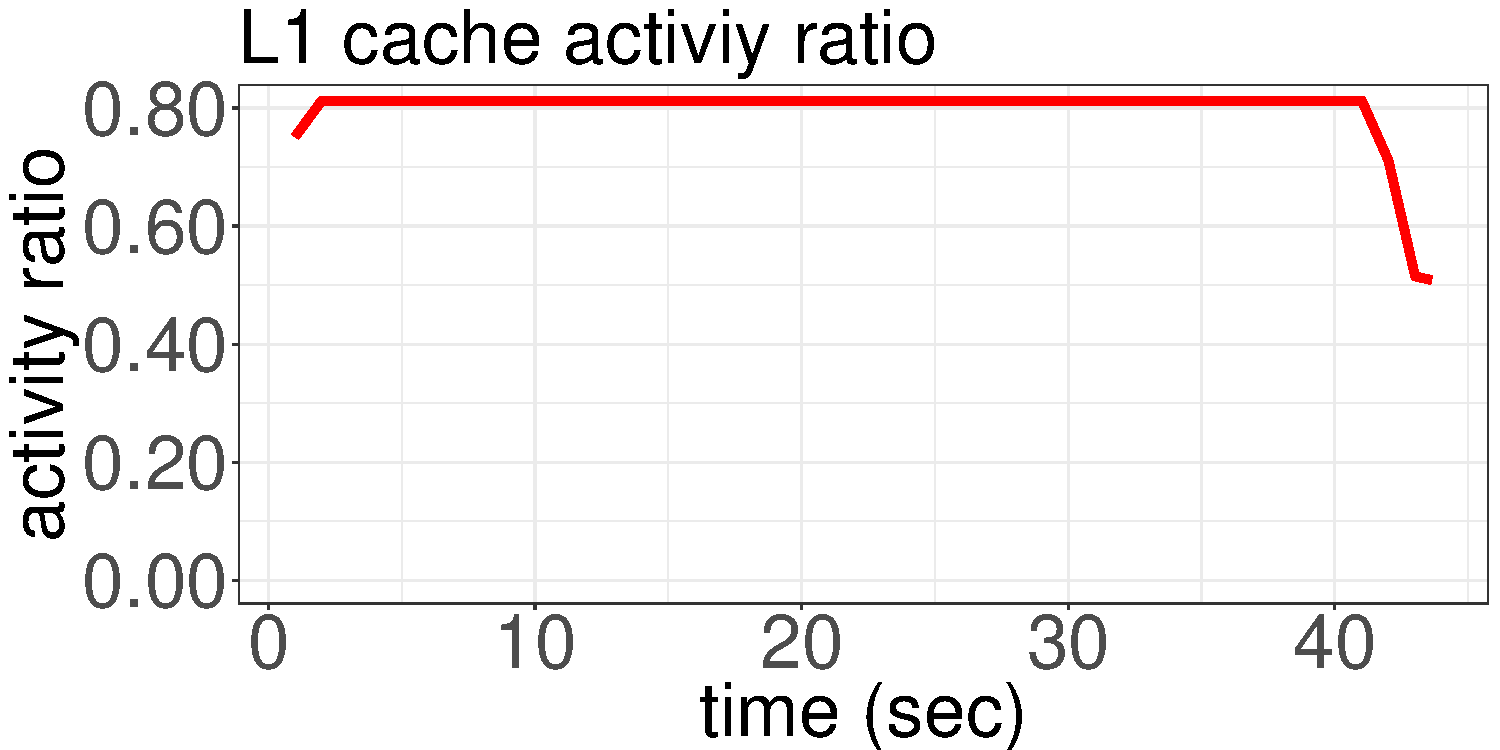
\includegraphics[width=\textwidth]{{power_aware_job_scheduling/figures/activity_ratios/lu-mz_C.16_MEM}.pdf}
	\end{subfigure}%
~
	\begin{subfigure}[b]{.48\textwidth}
	  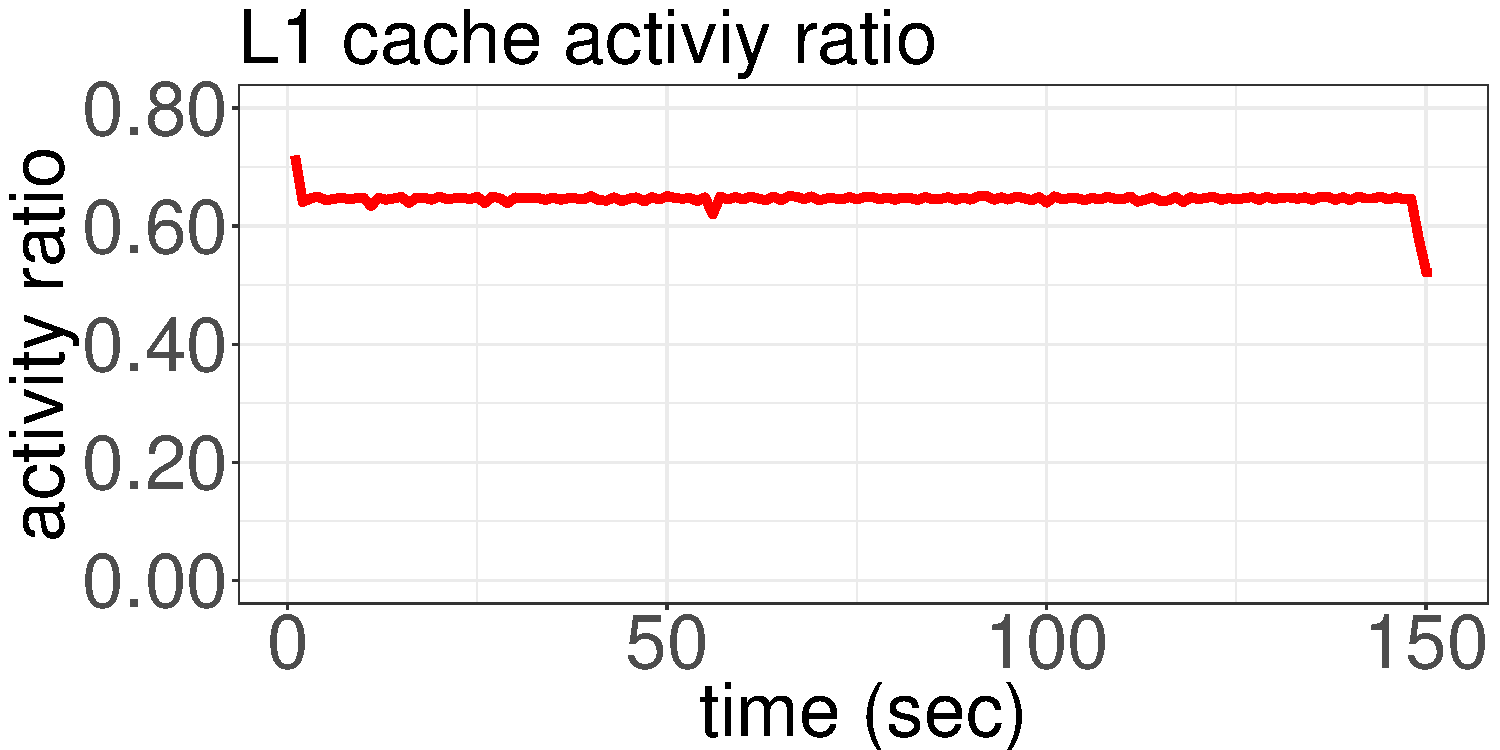
\includegraphics[width=\textwidth]{{power_aware_job_scheduling/figures/activity_ratios/sp-mz_D.8_MEM}.pdf}
	\end{subfigure}%
	\caption{Power, active cores and component activity ratio traces for MPI multi-node application, when running on 12 cores of a single socket. We show the activity on the socket running one the MPI processes.  PMC data is collected for all the processes and individual predictions are made for each socket.
 Architectural components shown are the fetch unit (FE), branch prediction unit (BPU)
					and L1 cache.  The activity ratios are the number of retired micro operations per unhalted cycle, relevant to each architectural component.
					In the case of cores, activity ratio is the number of active cores.  For memory the activity ratio is measured as the number of references (for caches) or LLC misses (for main memory) per cycle.} 
	\label{fig:component_activity_ratios_multi_node}
	\vspace{.5cm}
\end{figure*}



\begin{figure*}[p]
	\centering
	\begin{subfigure}[b]{.6\textwidth}
  	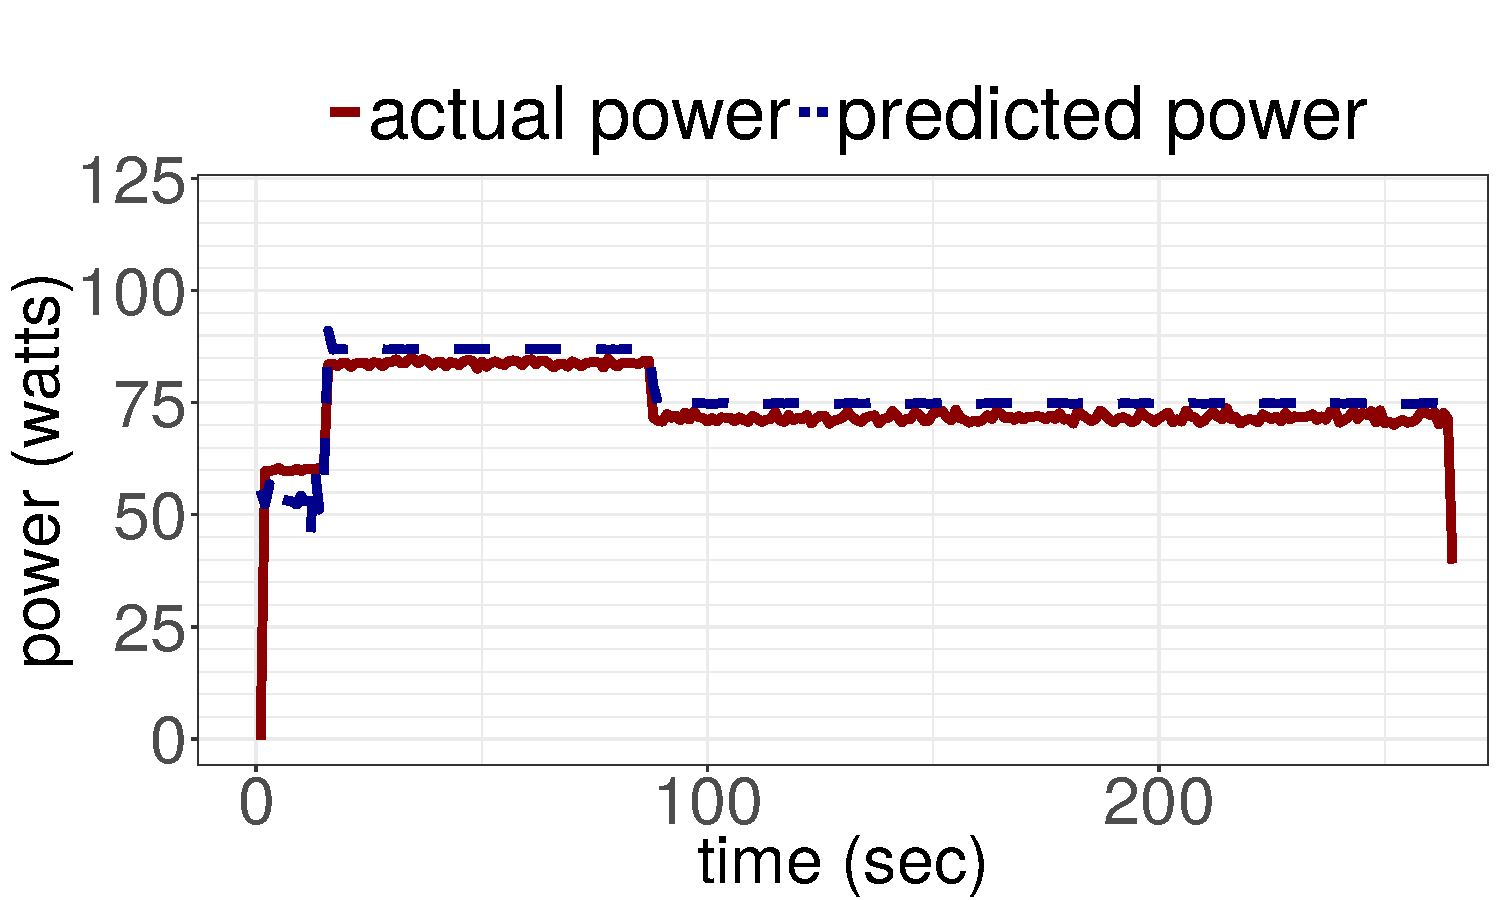
\includegraphics[width=\textwidth]{power_aware_job_scheduling/figures/predict_blackscholes_catalyst45}
  \end{subfigure}%
\qquad
	\begin{subfigure}[b]{.6\textwidth}
  	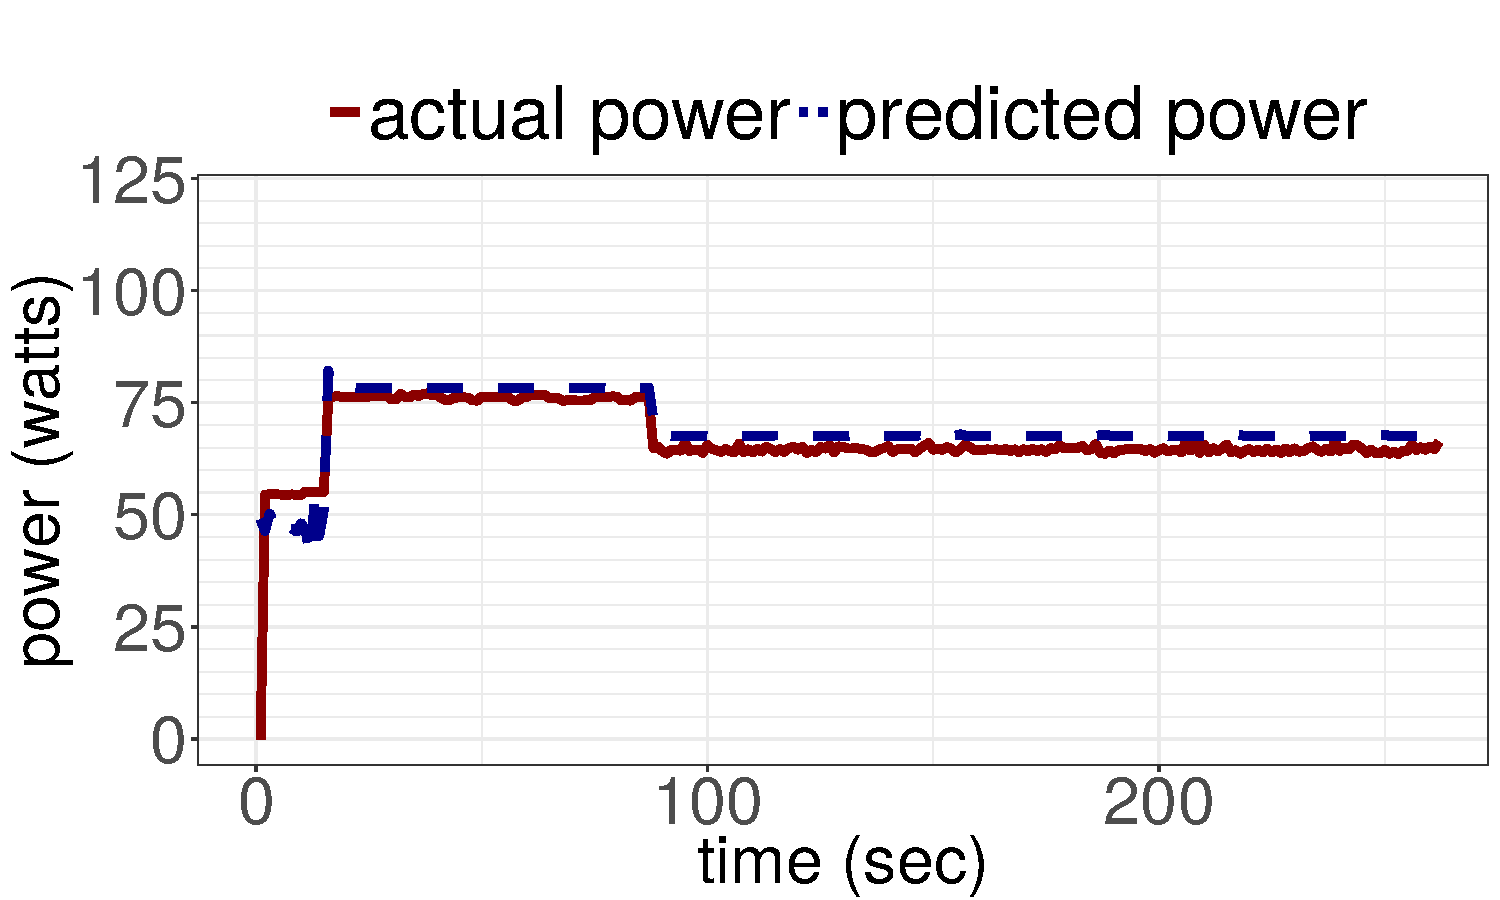
\includegraphics[width=\textwidth]{power_aware_job_scheduling/figures/predict_blackscholes_catalyst79}
	\end{subfigure}%
\qquad
	\begin{subfigure}[b]{.6\textwidth}
	  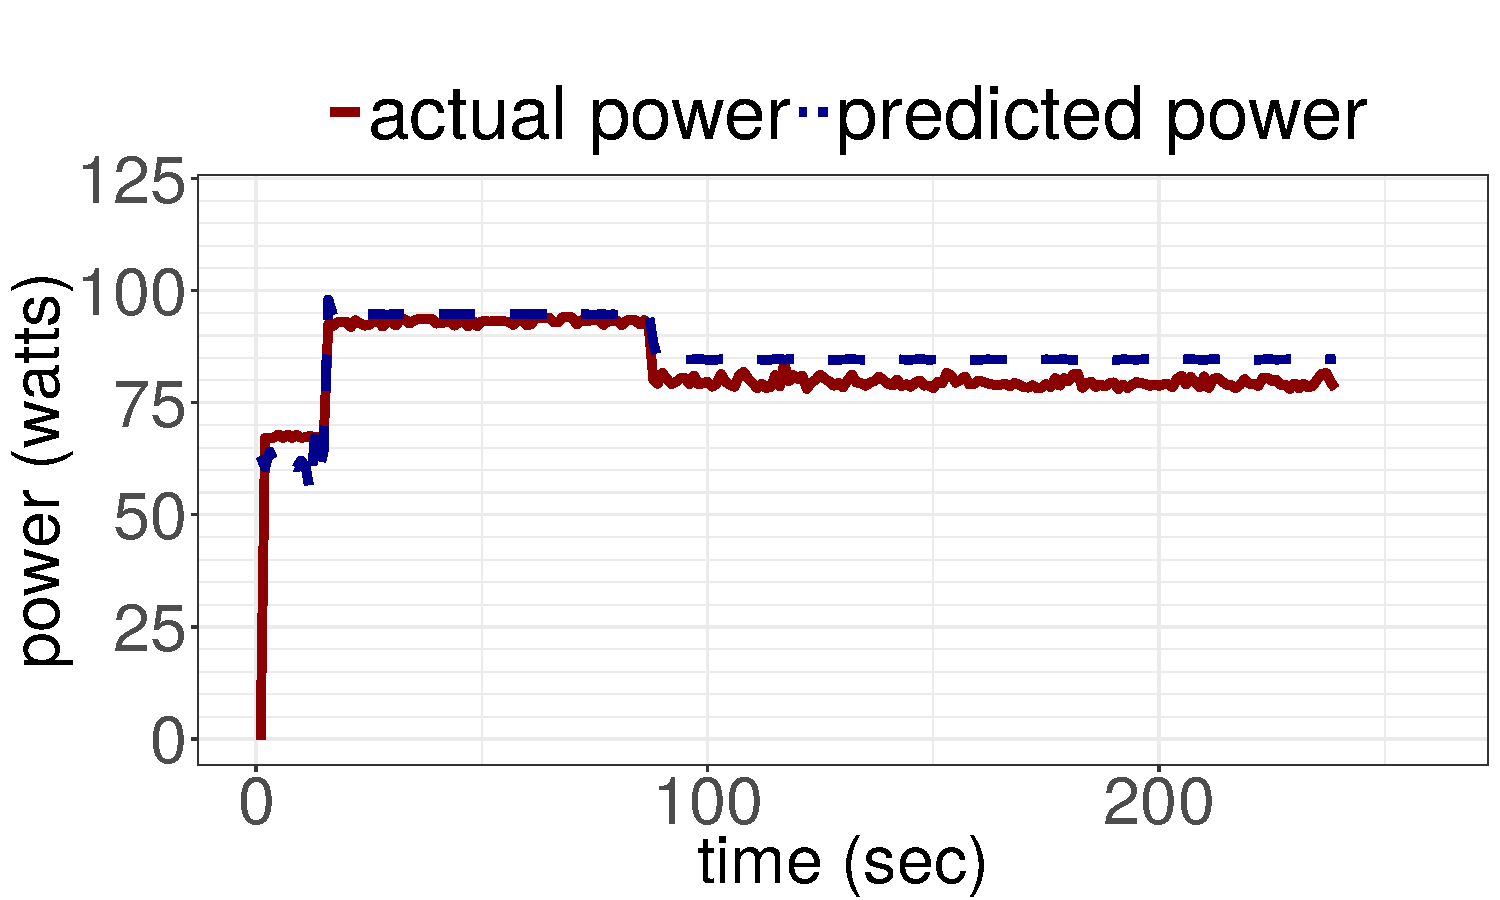
\includegraphics[width=\textwidth]{power_aware_job_scheduling/figures/predict_blackscholes_catalyst239}
	\end{subfigure}%

	\caption{Actual and predicted power consumption, using the PMC-based (Optimized PMC) model, for \textit{blackscholes} under three distinct sockets. Same CPU chip model is mounted on all three sockets, utilizing all 12 available cores.}
	\label{fig:prediction_eval}
	\vspace{.5cm}
\end{figure*}




Figures~\ref{fig:component_activity_ratios_single_node},\ref{fig:component_activity_ratios_multi_node} shows power and activity ratio profiles for the active cores (CORES), fetch unit (FE), branch predictor unit (BPU) and L1 cache, for the \textit{blackscholes}, \textit{bodytrack}, \textit{lu-mz\_C.16} and \textit{sp-mz\_D.8} parallel codes. 
For multi-node applications, \textit{lu-mz\_C.16} and \textit{sp-mz\_D.8}, we show the activity ratios and power consumption of one of the processes, running on one of the sockets.  
Each process has it's own set of activity ratios that result in individual predictions, per socket that the individual process run on.
The specific experimental setup to obtain these measurements is detailed in Chapter~\ref{chap:methodology}. 
All applications have a unique power profile that is the result of the different component activity ratios.  
For example, \textit{blackscholes} and \textit{sp-mz\_D.8} have high FE and CORES activity that contribute to the power consumption.
However, \textit{blackscholes} has minimal activity in L1 cache, which results in lower overall power consumption, when compared to \textit{sp-mz\_D.8}.
Moreover, \textit{lu-mz\_C.16} has similar activity ratios to \textit{sp-mz\_D.8} but significantly lower activity in cores (only uses 1 core per process), which
results in lower power consumption.  Finally, we can observe how changes in component activity influences power consumption in the cases of \textit{blackscholes}
and \textit{bodytrack}.

We then align the activity ratios with measured power data, which allows us to express
the power of an application on a particular socket as: 
%Per each instant of time we can map the activity ratios values to the measured power in that same instant of time. 
%Thus, power 
%model the power of an applicatiopn 
%can be express the relative to the activity ratios of all architectural components:
\begin{equation}
\label{eq:model_formula}
%MS: changed to c for "cores", so we have "i" free for socket_i (socket_n sounds too much like number of sockets or like the last socket)
P = AC * W_{cores} + \sum_{c=1}^{N_{comp}} ( AR_c * W_c )
\end{equation}
where $AR_i$ is the activity ratio of power component $i$, $AC$ is the average number of active cores and $P$ is the power consumption, at a given moment. 
These values are known for any given application in our training set.  
However, we need to find the contribution of each component to the total power consumption $P$.  
This is expressed using a set of weights, denoted as $W_i$ for architectural component $i$ and $W_{cores}$ for active cores.

We determine the weights
%To generate a per socket model that captures its inherent power variability, 
%we first need to obtain data from some training runs.  
%During this 
using a
training stage during which we monitor power along with the architectural component activity for a small set of kernels.  The choice of training benchmarks should reflect different application behaviors (e.g., computation vs. memory bound) and stress different architectural components, such as integer or floating point units, in addition to
the different memory levels.  
The list of applications used for training can be found in Table~\ref{tab:training_set}. 
To better account for the power contribution of the memory subsystem, this list includes an additional synthetic code, \textit{mem\_bench}, a microbenchmark that causes misses on different levels of the memory hierarchy. %complementing the kernels in our training set.

With the data measured in this training stage, we then use
%By means of 
linear regression to determine the values of $W_i$ and $W_{cores}$ that best fit in Equation~\ref{eq:model_formula}
%according to the data obtained while running the training kernels represented in Table~\ref{tab:training_set} 
on a given socket.  
The resulting linear model is socket-specific and can predict the power consumption of a generic application assuming its activity ratios for all architectural components and cores are known.

%Until this point, we regard the system as homogeneous in terms of power consumption.  
Due to manufacturing variability, power consumption differs between sockets, which means that  $W_c$ and $W_{cores}$ are socket-specific and obtained by
%When 
solving Equation~\ref{eq:model_formula} individually for each socket.
%, we get per socket $W_{cores}$ and $W_i$ values.
In terms of the activity ratio values per application, we assume them to be invariant across all sockets featuring the same architectural design.
Consequently, the socket-specific Formula~\ref{eq:model_formula} can be extended to integrate all sockets featuring the same architectural design: 
\begin{equation}
\label{eq:model_variability_formula}
P_{socket_i}^{app} = AC^{app} * W_{cores}^{socket_i} + \sum_{c=1}^{N_{comp}} ( AR_c^{app} * W_c^{socket_i} )
\end{equation}
%In terms of performance though, the system is homogeneous, thus its safe to assume that the activity ratios for the  architectural components and number of active cores is the same on all sockets.
From this formula we can obtain a power prediction of an application running on any chosen socket, which is characterized in terms of its weights.
%, and thus capture the per socket manufacturing variability;
%Homogeneous parallel systems just require a single linear model expressed in terms of Formula~\ref{eq:model_variability_formula}.
%Heterogeneous systems need a different model per each different socket architecture they integrate.
For each parallel code we just need a single run on a generic socket to compute $AR_c$ and $AC$, which are socket-independent as they are determined by the architectural design.
%\par  
%It is also crucial that the training data captures different application behaviors (e.g. computation/memory bound).  
%We also need to stress different architectural components, preferably not in the same kernel, such as integer, floating point and vectorized operations in addition to 
%the different memory levels.  The list of applications used for training can be found on Table \ref{tab:training_set}.
%Isolating architectural components is not always trivial, such as the memory system.
%To isolate the power contribution of the memory subsystem, we design \textit{mem\_bench}, a microbenchmark that causes misses on different levels of the memory hierarchy, complementing the kernels in our training set.
%\par
For multi-node applications, individual predictions need to me made for each socket an MPI process is run on.  A corresponding model needs to be applied to each socket, 
which has been trained for each socket individually, producing a different set of weights.  
The resulting prediction is a set of predictions, equal to the number of sockets the application run on, each prediction accounting for the individual socket's own variability. 

Figure~\ref{fig:prediction_eval} shows power profiles of the \textit{blackscholes} code (solid line) running on three different sockets, together with the corresponding predicted power consumption (dashed line).
Details on the machine and execution setup can be found in Chapter~\ref{chap:methodology}.  
Figure~\ref{fig:prediction_eval} displays how the power consumption varies up to 19\% for the same application (from 76W to 96W peak power), depending on the socket it runs on.
The predicted values capture the power consumption variability for all cases. 

We denote the model using all architectural components listed in Table~\ref{tab:comp_formulas} along with the number of active cores as the \textit{Generic PMC Model}.
%A more detailed evaluation and validation of this model is presented in Section~\ref{sec:results}, where two variations of it are examined.
We also consider a second model that uses, per each application, the subset of architectural components that provides the most accurate results.  
All possible combinations of architectural components are considered and a prediction error is computed for each one.  
We use the Mean Absolute Percentage Error (MAPE) formula for computing this prediction error
\begin{equation}
\label{eq:mape}
M = \frac{100}{n}\sum^{n}_{t=1}|\frac{A_t - F_t}{A_t}|
\end{equation}
where $A_t$ and $F_t$ are the actual and predicted values for observation $t$, and $n$ is the total number of observations. 
The model with the lowest error value is chosen for all future predictions. 
This tuning process can be done offline per each targeted application using data obtained from a single parallel execution.
We denote the model resulting from this methodology as the \textit{Optimized PMC Model}.
Section~\ref{sec:model_validation} shows a detailed evaluation and validation of all considered models.
